\documentclass{article}
\usepackage[T1,T2A]{fontenc}
\usepackage[utf8]{inputenc}
\usepackage[english,russian]{babel}

\usepackage[left=3cm,right=3cm,
    top=3cm,bottom=3cm,bindingoffset=0cm]{geometry}

\usepackage{graphicx}
\usepackage{color}
\usepackage{hyperref}
\usepackage{amsmath}

\usepackage{setspace}
\usepackage{indentfirst}
\usepackage{textcomp}
\usepackage{ifthen}
\usepackage{calc}

\title{Теория Вероятностей и Математическая Статистика\\
ФИИТ, 2 курс, 4 семестр}
\author{Лекция 3}

\begin{document}
\maketitle

\section {Формула полной вероятности}

Наша основная тема на сегодня -- формула полной вероятности.
Мы будем рассматривать ситуации, когда опыт производится сложным образом и содержит слишком много составляющих.

\quad

Итак, допустим мы имеем изначально множество исходов опыта $\Omega$. Это множество можно разделить на некоторые части $(H_1, H_2 \ldots)$, а мы хотим рассмотреть некоторое событие $A$, которое так же является подмножеством $\Omega$ (по определению).

\begin{center}
    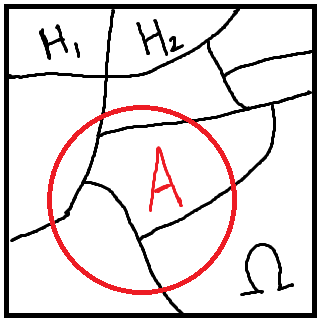
\includegraphics[scale=0.6]{1.png}
\end{center}

Мы можем составить набор событий (которые мы будем называть \textbf{гипотезы}): $H_1, H_2, \ldots, H_n, \ldots$

Этот набор удовлетворяет следующим условиям:

\begin{enumerate}
\item События попарно: $H_iH_j = \emptyset\quad (i \not= j)$
\item События образуют полную группу: $H_1 + H_2 + \ldots + H_n + \ldots = \Omega$
\end{enumerate}

Таким образом мы получаем набор гипотез -- полная группа попарно несовместных событий, которая построена до опыта -- априорти. А наше некоторое событие $A$ можно представить как объединение этих групп:

$$ A = A  \Omega = A (H_1 + H_2 + \ldots) = AH_1 + AH_2 + \ldots$$

Очевидно, то слагаемые будут, как и гипотезы, попарно несовместны. Тогда можно перейти к нахождению вероятности через сумму вероятностей:

$$ P(A) = P(A\Omega) = P(A(H_1 + H_2 + \ldots)) = P(AH_1) + P(AH_2) + \ldots) $$

А далее к каждому слагаемому применим теорему умножения:

$$ = P(H_1)P(A|H_1) + P(H_2)P(A|H_2) + \ldots $$

Таким образом мы получили \textbf{формулу полной вероятности}:

$$ P(A) = \sum\limits_{i = 1}^\infty P(H_i)P(A|H_i) $$

\subsection{Пример}

Три станка изготавливают одинаковые детали. Вероятность брака составляет $0.01, 0.02, 0.03$ соответственно. На 1-м станке изготовленно 2000 деталей, на 2-м -- 3000, а на 3-м 5000. ОТК берет на контроль одну из всех выпущенных деталей. Найти вероятность того, что эта деталь -- годная.
\\

Первое, что стоить отметить, что задача -- многонаправленная (и производство есть, и отбор). Если не брать в рассчет годная ли деталь, можно отметить, что любая деталь будет изготовленна на одном из станков. Значит можно выделить следующие события:
\\

$H_1 = \{$ взятая деталь изготовлена на 1-м станке $\}$

$H_2 = \{$ взятая деталь изготовлена на 2-м станке $\}$

$H_3 = \{$ взятая деталь изготовлена на 3-м станке $\}$
\\

При этом общее количество деталей равно: $N = 10000$. А мы можем вычислить вероятности описанных событий (дроби сокращать не будем, так как одинаковые знаменатели могут в будущем упростить жизнь):
\\

$P(H_1) = \frac{2000}{10000} = \frac{2}{10}$\qquad$P(H_2) = \frac{3000}{10000} = \frac{3}{10}$
\qquad$P(H_3) = \frac{5000}{10000} = \frac{5}{10}$
\\

На что можно обратить внимание: если мы построили события правильно, то они должны составлять полную группу, а значит и сумма вероятностей должна быть равна единице (что у нас работает).

Далее поинтересуемся, с каким качеством изготовлена деталь. Построим следующее событие:
\\

$A = \{$ изготовленная деталь годная $\}$
\\

Тогда можем построить условные вероятности:
\\

$P(A|H_1) = 0,99$\qquad$P(A|H_2) = 0,98$\qquad$P(A|H_3) = 0,97$
\\

По условию нам надо найти просто полную вероятность, так что воспользуемся \textbf{формулой полной вероятности}:
\\

$P(A) = P(H_1)P(A|H_1) + P(H_2)P(A|H_2) + P(H_3)P(A|H_3) = \frac{2}{10} \cdot 0.99 +  \frac{3}{10} \cdot 0.98 +  \frac{5}{10} \cdot 0.97 = \ldots$


\section{Формула Байеса}

Допустим, мы проделали следующие шаги:

\begin{enumerate}
\item До опыта построены гипотезы
\item Провели опыт (событие $A$ реализовалось, либо нет) // Для себя примем, что произошло событие $A$ произошло (если нет, то произошло $\overline{A}$)
\end{enumerate}

Возникает вопрос: как изменятся вероятности гипотез после проведения опыта. Рассмотрим следующую вероятность некоторой гипотезы $H_k$:

$$P(H_k | A) = \frac{P(H_kA)}{P(A)} = \frac{P(H_k)P(A|H_k)}{\sum\limits_{i = 1}^\infty P(H_i)P(A|H_i)}\qquad,k=1,2,\ldots$$

Эта запись и называется Формулой Байеса. Она позволяет учесть в опыте произошедшее событие $A$.

\subsection{Пример}

Из 30 экзаменационных билетов студент выучил 10. Какова вероятность, что ему попадется нужный билет?
\\

Если он вышел первый ($A$), тогда вероятность достать билет: $P(A) = \frac{10}{30} = \frac{1}{3}$.

Если он вышел второй, но все выученные билеты все еще лежат на столе, то получаем условную вероятность: $P(A|B) = \frac{10}{29}$

$\ldots$

\subsection{Пример (продолжение 1.1)}

Взятая ОТК деталь годная. Найти вероятность того, что эта деталь изготовленна на 3-м станке.
\\

У нас имеются следующие события:

$H_3 = \{$ взятая деталь изготовлена на 3-м станке $\}$

$A = \{$ изготовленная деталь годная $\}$
\\

Тогда нам надо найти следующую вероятность, воспользуясь Формулой Байеса:

$$ P(H_3 | A) = \frac{P(H_3)P(A|H_3)}{P(A)} =
\frac{\frac{5}{10} \cdot 0.97}{\frac{2}{10} \cdot 0.99 +  \frac{3}{10} \cdot 0.98 +  \frac{5}{10} \cdot 0.97} = \frac{5 \cdot 97}{2 \cdot 99 + 3 \cdot 98 + 5 \cdot 97} = \ldots$$

\section{Схема независимых опытов / Схема Бернулли}

Одна из самых важных частей Теории Вероятностей -- Схема Бернулли.

В одних и тех же условиях один и тот же опыт повторяется $n$ раз. В каждом из случаев мы имеем один из двух исходов: $A$ реализовалось, либо $\overline{A}$ реализовалось.

\begin{center}
    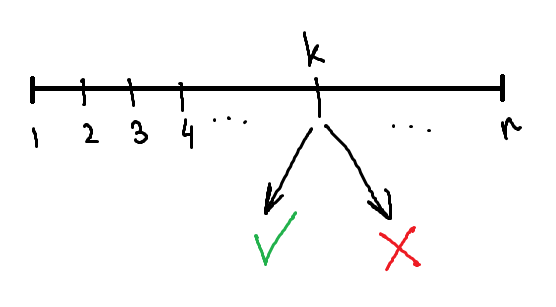
\includegraphics[scale=0.6]{2.png}
\end{center}

Если событие $A$ реализовалось, мы говорим, что в одном отдельно взятом опыте произошел успех. Вероятность обозначим следующим образом: $P(A) = p$.

Вероятность реализации события $\overline{A}$ (неуспех) обозначим следующим образом: $P(\overline{A}) = 1 - p = q$
\\

Нас же будет интересовать следующее: какова вероятность того, что в последовательности из $n$ опытов "успех" будет зафиксирован $m$ раз (где $0 \leq m \leq n$).

Рассмотрим следующую ситуацию. Пусть у нас имеется $m$ успехов, и все они расположены в начале друг за другом: (1)

\begin{center}
    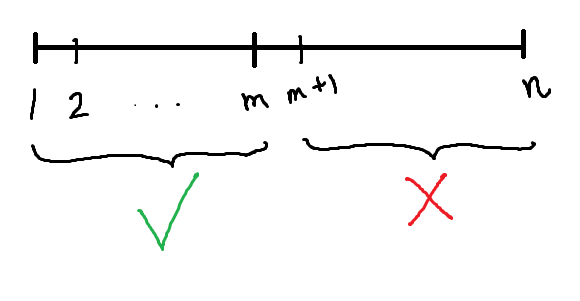
\includegraphics[scale=0.6]{3.png}
\end{center}

Тогда для нашей картины найти вероятность достаточно просто в силу независимости опытов:

$$P(A\ldots A\cdot\overline{A}\ldots\overline{A}) = p^m \cdot q^{n - m}$$

Но в нашем вопросе нас будет интересовать количество успехов, а не место их расположения. То есть требуется выбрать не первые $m$ мест, а произвольные $m$ мест. Тогда количество таких способов мы тоже знаем, как подсчитывается: $C_n^m$ (сочетания из $n$ по $m$). Таким образом, получаем следующую вероятность "$m$ успехов среди $n$ опытов":

$$P_n(m) = C_n^m p^m \cdot q^{n - m} $$

Полученное выражение является формулой Бернулли.

\subsection{Пример}

Бросают 3 монеты. Найти вероятность выпадения одного герба.
\\

Имеем событие:

$A = \{$ выпал 1 герб $\}$ -- один "успех" в серии из 3-х опытов:

$$P_3(1) = C_3^1 \cdot \Biggl(\frac{1}{2}\Biggr)^1 \Biggl(\frac{1}{2}\Biggr)^{3 - 1} = 3 \cdot \frac{1}{2} \cdot \frac{1}{4} = \frac{3}{8}$$

\subsection{Пример}

Что вероятнее: выиграть у равносильного партнера 3 партии из 4, или 5 партий из 8. (Без ничьих!).

"успех"\quad3 из 4 ($75\%$)

"успех"\quad5 из 8 ($62.5\%$)

Мы же склоняемся к тому, что более "скромный" успех достижим. Тогда сравним следующие вероятности:
$P_3(4)$ и $P_8(5)$. Построим отношение:

$$ \frac{P_4(3)}{P_8(5)} = \frac{C_4^3 \cdot (\frac{1}{2})^3 (\frac{1}{2})^{4 - 3}}
{C_8^5 \cdot (\frac{1}{2})^5 (\frac{1}{2})^{8 - 5}} = \frac{4\cdot (\frac{1}{2})^4}{\frac{2 \cdot 8 \cdot 7 \cdot 6}{6} \cdot (\frac{1}{2})^8} = \frac{16}{14} = \frac{8}{7} > 1$$

Таким образом, мы явно показали, что "скромный" результат вероятен меньше. Однако, это вполне логично. Ту же ситуацию мы можем посмотреть в другой ситуации: легче добиться успеха в стометровке или 40 километровом марафоне? Тут уже вполне очевидно, что в стометровке просто надо выложиться один раз в короткий промежуток, в отличии от марафона, где даже в легком режиме можно просто не дойти.

\section{Полиномиальная схема}

Это расширение схемы Бернулли. Теперь у нас ситуация выглядит похожим образом: имеем последовательность независимых опытов, и в каком-то опыте $k$ у нас может произойти событие $A_1$, или событие $A_2$, или событие $A_m$. При этом эти события образуют полную группу попарно несовместных событий.

\begin{center}
    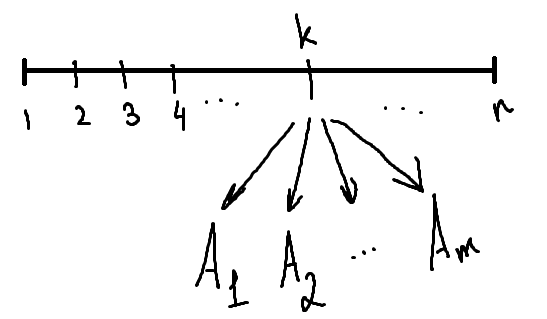
\includegraphics[scale=0.5]{4.png}
\end{center}

$$P(A_1) = p_1,\qquad P(A_2) = p_2, \qquad \ldots \qquad P(A_m) = p_m$$

$$ p_1 + p_2 + \ldots + p_m = 1$$

И для разбора таких ситуаций имеем:

$$P_n(n_1, n_2, \ldots, n_m) = \frac{n!}{n_1!n_2!\ldots n_m!} P_1^{n_1} P_2^{n_2} \ldots P_m^{n_m} $$

Эта запись и есть та самая полиномиальная формула.

\subsection{Пример}

На интервале $(1; 5)$ наугад выбирают 5 точек. Нужно найти вероятность

\begin{enumerate}
\item В интервале $(1; 2)$ и $(3; 5)$ окажется 2 и 3 точки соответственно
\item В интервале $(1; 3)$ и $(2; 5)$ окажется равное количество точек
\end{enumerate}
\\

1) Можно отметить, что вероятности мы рассчитываем геометрически. То есть попасть именно в точку $1$ можно с нулевой вероятностью. А попасть в интервал можно с вероятностью отношения длины интервала к всему интегвалу. Тогда получается, что вероятность попасть в интервал $(1; 2)$ равна $\frac{1}{4}$, а в интервал $(3; 5)$ равна $\frac{2}{4}$.

Однако наши вероятности не образуют полную группу (сумма вероятностей не равна $1$). Можем решить эту проблему добавлением интервала $(2; 3)$, для которого вероятность будет $\frac{1}{4}$. Так мы образуем полную группу.

Нас интересует следующее распределение точек:

$$ P_5(2, 0, 3) = \frac{5!}{2! 0! 3!}\Biggl(\frac{1}{4}\Biggr)^2 \Biggl(\frac{1}{4}\Biggr)^0 \Biggl(\frac{2}{4}\Biggr)^3 = \frac{5 \cdot 4}{2} \cdot \frac{2^3}{4^5} = \ldots$$
\\

2) Для этого пункта у нас ситуация немного другая. Интервалы получились $(1; 3)$ и $(2; 5)$. И длина у них разная, количество точек должно быть равное.

Однако, если учесть, что колво точек всего у нас нечетное ($5$), а интервалы пересекаются, то в пересечении может быть $1$ точка, $3$ точки или $5$ точек. Таким образом, получаем следующие случаи:

$$P_5(2, 1, 2)\qquad P_5(1, 3, 1)\qquad P_5(0, 5, 0)$$

Таким образом, надо найти сумму вышеприведенных вероятностей:

$$P_5(2, 1, 2) + P_5(1, 3, 1) + P_5(0, 5, 0) = $$
$$\Biggl[\frac{5!}{2! 1! 2!}\Bigl(\frac{1}{4}\Bigr)^2 \Bigl(\frac{1}{4}\Bigr)^1 \Bigl(\frac{2}{4}\Bigr)^2\Biggr] +
\Biggl[\frac{5!}{1! 3! 1!}\Bigl(\frac{1}{4}\Bigr)^1 \Bigl(\frac{1}{4}\Bigr)^3 \Bigl(\frac{2}{4}\Bigr)^1\Biggr] +
\Biggl[\frac{5!}{0! 5! 0!}\Bigl(\frac{1}{4}\Bigr)^0 \Bigl(\frac{1}{4}\Bigr)^5 \Bigl(\frac{2}{4}\Bigr)^0\Biggr] = \ldots$$

\section{Пример (для формулы полной вероятности)}

Имеется 2 урны: первая содержит 2 белых и 3 черных шара, а вторая 3 белых и 4 черных.

Ситуация следующая: наугад выбрана урна из нее наугад взят шар, оказавшийся белым. Нужно найти вероятность того, что второй шар взятый из той же урны окажется так же белым.
\\

Самое существенное в данном условии то, что взятый шар оказался белым. Это означает, что в нашем опыте есть событие, которое произошло, поэтому вероятность, которую мы ищем, точно условная.
\\

Посмотрим, какие события мы можем здесь рассмотреть:
\\

$H_1 = \{$ шар взят из первой урны $\}$

$H_2 = \{$ шар взят из второй урны $\}$

$P(H_1) = P(H_2) = \frac{1}{2}$ (до проведения опыта)

Также имеем:
\\

$A = \{$ первый шар белый $\}$

$B = \{$ второй шар белый $\}$
\\

\textbf{Примечание.} Как всегда мы сначала описываем задачу. Нахождением, вычислениями и остальные размышления мы делаем на следующем этапе.
\\

Требуемая вероятность:

$$P(B | A) = \frac{P(AB)}{P(A)}$$

По формуле полной вероятности получим:

$$ = \frac{P(H_1) P(AB|H_1) + P(H_2) P(AB|H_2)}{ P(H_1) P(A|H_1) + P(H_2) P(A|H_2)}
= \frac{\frac{1}{2}\cdot\frac{2}{5}\cdot\frac{1}{4} + \frac{1}{2}\cdot\frac{3}{7}\cdot\frac{2}{6}}
{\frac{1}{2}\cdot \frac{2}{5} + \frac{1}{2} \cdot \frac{3}{7}} = \ldots$$
\\

Вообще говоря, можно было бы применить формулу полной вероятности напрямую, но это было бы достаточно сложно вычислять, так как полученные вероятности были бы условными, в том числе условные вероятности гипотез:

$$P(B|A) = P(H_1|A) \cdot P(B|AH_1) + P(H_2|A) \cdot P(B|AH_2)$$

\end{document}
